\definecolor{C1}{RGB}{226, 43, 41}
\definecolor{C2}{RGB}{47, 96, 206}
\definecolor{C3}{RGB}{246, 175, 11} 


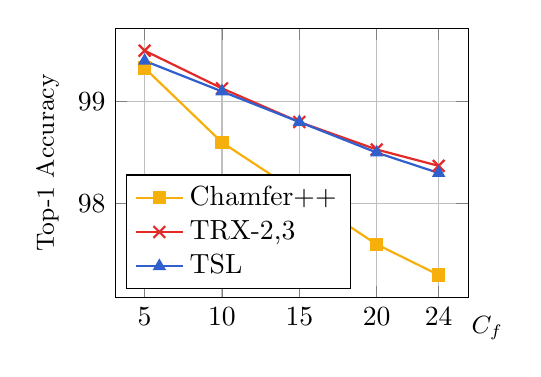
\begin{tikzpicture}
  \begin{axis}[
    width=0.5\linewidth,
    height=5cm, 
    xtick = {5,10,15,20,24},
	legend cell align={left},
	legend pos=south west,
    grid=both,
    ylabel={\small Top-1 Accuracy},
    xlabel={\small $C_f$},
    xlabel style={yshift=10pt, xshift=80pt,anchor=north east},
  ]
\addplot [thick, color=C3, mark=square*,  mark size=2] coordinates {(5, 99.33)(10, 98.6)(15, 98.1)(20, 97.6) (24, 97.3)};
\addlegendentry{Chamfer++} 

\addplot [thick, color=C1, mark=x,  mark size=3] coordinates {(5, 99.5) (10, 99.13) (15, 98.8) (20, 98.53) (24, 98.37)};   
\addlegendentry{TRX-{2,3}} 

\addplot [thick, color=C2, mark=triangle*,  mark size=2] coordinates {(5, 99.4) (10, 99.1) (15, 98.8) (20, 98.5) (24, 98.3)};     
\addlegendentry{TSL} 

  \end{axis}
\end{tikzpicture}